\documentclass{bmcart}

%%%%%%%%%%%%%%%%%%%%%%%%%%%%%%%%%%%%%%%%%%%%%%
%%                                          %%
%% CARGA DE PAQUETES DE LATEX               %%
%%                                          %%
%%%%%%%%%%%%%%%%%%%%%%%%%%%%%%%%%%%%%%%%%%%%%%

%%% Load packages
\usepackage{amsthm,amsmath}
\usepackage{graphicx}
%\RequirePackage[numbers]{natbib}
%\RequirePackage{hyperref}
\usepackage[utf8]{inputenc} %unicode support
%\usepackage[applemac]{inputenc} %applemac support if unicode package fails
%\usepackage[latin1]{inputenc} %UNIX support if unicode package fails
\usepackage[utf8]{inputenc}
\usepackage[english]{babel}
\usepackage{xspace,color}
\definecolor{dkgreen}{rgb}{0,0.6,0}
\definecolor{gray}{rgb}{0.5,0.5,0.5}
\definecolor{mauve}{rgb}{0.58,0,0.82}
\usepackage{url}
\usepackage{listings}
\lstset{ %
  language=R,                     % the language of the code
  basicstyle=\footnotesize,       % the size of the fonts that are used for the code
  numbers=left,                   % where to put the line-numbers
  numberstyle=\tiny\color{gray},  % the style that is used for the line-numbers
  stepnumber=1,                   % the step between two line-numbers. If it's 1, each line
                                  % will be numbered
  numbersep=5pt,                  % how far the line-numbers are from the code
  backgroundcolor=\color{white},  % choose the background color. You must add \usepackage{color}
  showspaces=false,               % show spaces adding particular underscores
  showstringspaces=false,         % underline spaces within strings
  showtabs=false,                 % show tabs within strings adding particular underscores
  frame=single,                   % adds a frame around the code
  rulecolor=\color{black},        % if not set, the frame-color may be changed on line-breaks within not-black text (e.g. commens (green here))
  tabsize=2,                      % sets default tabsize to 2 spaces
  captionpos=b,                   % sets the caption-position to bottom
  breaklines=true,                % sets automatic line breaking
  breakatwhitespace=false,        % sets if automatic breaks should only happen at whitespace
  title=\lstname,                 % show the filename of files included with \lstinputlisting;
                                  % also try caption instead of title
  keywordstyle=\color{blue},      % keyword style
  commentstyle=\color{dkgreen},   % comment style
  stringstyle=\color{mauve},      % string literal style
  escapeinside={\%*}{*)},         % if you want to add a comment within your code
  morekeywords={*,...}            % if you want to add more keywords to the set
} 

\begin{document}

	\begin{frontmatter}
	
		\begin{fmbox}
			\dochead{Research}
			
		
			\title{Red de los targets de SARS-CoV2}
			
		
			\author[
			  addressref={aff1},                  
			  corref={aff1},                    
			  email={sandra091999@gmail.com}  
			]{\inits{S.C.L}\fnm{Sandra} \snm{Castro Labrador}} 
			\author[
			  addressref={aff1},                 
			  corref={aff1},                      
			  email={fiorellapiriz@uma.es}    
			]{\inits{F.P.S}\fnm{Fiorella} \snm{Piriz Sapio}} 
			\author[
			  addressref={aff1},                 
			  corref={aff1},                      
			  email={adrianseor.99@gmail.com}   
			]{\inits{A.S.O}\fnm{Adrián} \snm{Segura Ortiz}} 
		    \author[
			  addressref={aff1},                   
			  corref={aff1},                      
			  email={Rvalpalacios@gamil.com}  
			]{\inits{MR.V.P}\fnm{María del Rocío} \snm{Valderrama  Palacios}}
			
	
			\address[id=aff1]{%                           
			  \orgdiv{ETSI Informática},             
			  \orgname{Universidad de Málaga},          
			  \city{Málaga},                              
			  \cny{España}                                    
			}
		
		\end{fmbox}
		
		\begin{abstractbox}
		
			\begin{abstract}
			En el presente proyecto de investigación procederemos a explorar las diversas interacciones que existen entre las proteínas humanas y las 29  proteínas conocidas que codifican el virus SARS-CoV-2. Con el fin de alcanzar este objetivo, realizaremos un intenso trabajo de recopilación de material bibliográfico acerca cómo interacciona el organismo comentado sobre el interactoma humano. Estos datos los podemos encontrar en artículos y libros en los que los experimentos realizados tienen como objetivo determinar e mapa de interacción de las proteínas humanas con las proteínas del SARS-Cov-2. En cuanto a la herramienta para obtener la red del sistema, emplearemos principalmente STRING y R, puesto que ya hemos visto a lo largo del curso la cantidad de información relevante que nos pueden proporcionar. 
	
			\end{abstract}
			
		
			\begin{keyword}
			\kwd{ SARS-CoV-2}
			\kwd{interactoma humano}
			\kwd{STRING}
			\kwd{R}
			\end{keyword}
		
		
		\end{abstractbox}
	
	\end{frontmatter}
	

	%%%%%%%%%%%%%%%%%%%%%%%%%%%%%%%%%
	%% COMIENZO DEL DOCUMENTO REAL %%
	%%%%%%%%%%%%%%%%%%%%%%%%%%%%%%%%%
	
	\section{Introducción}

A finales de 2019 se unió a la familia de los coronavirus el denominado síndrome respiratorio agudo severo coronavirus 2 (SARS-CoV2), cuya infección da lugar al conocido coronavirus 2019 o COVID-19. Este virus ha provocado una pandemia y crisis mundial, dejando por delante un total de más de 2 millones de muertes y casi 96 millones de infectados en todo el mundo. Por ello, desde los equipos de investigación, se está trabajando inmensurablemente por identificar los componentes del mismo, así como sus genes, sus proteínas y las formas en las que estas interaccionan con el ser humano. 

A día de hoy se sabe que el SARS-CoV-2 está formado por 29 proteínas que se asocian con las células humanas dando lugar a múltiples de síntomas que en su máxima expresión pueden llevar a la muerte del individuo con relativa facilidad.

Por otra parte, debemos tener tener en cuenta que el interactoma define el conjunto de interacciones moleculares que tiene lugar en el interior de una célula. El estudio de estas redes biológicas es realmente relevante en diversas áreas de investigación, ya que conocer cómo interaccionan las proteínas entre sí (PPI) permite el descubrimiento de patrones, la elaboración de fármacos o la explicación de procesos biológicos, entre otros.

Es por ello, por lo que en este proyecto pretendemos modelar y estudiar la red de interacción de las proteínas de este virus con las proteínas humanas, así como examinar brevemente si existe algún conjunto de fármacos con targets en las proteínas de la red, observar si la combinación de medicamentos afecta a las enzimas virales, determinar las funciones celulares a las que afecta, etc.
 
Finalmente, tanto los resultados como la presente memoria,  serán proporcionados en el repositorio de github de la asignatura, accesible a todos los miembros del grupo.

	\section{Materiales y métodos}
\subsection{Carga de datos}
El primer paso para poder modelar y análizar nuestra red es descargar los datos desde StringDB.
Hemos obtenido la red de 332 mencionada por Gordon et al en la versión web de StringDB, ampliando el número de proteínas en la segunda capa hasta obtener una red completamente conectada, que hemos descargado en formato tsv. Este archivo lo hemos usado posteriormente para cargar la red en nuestro entorno de trabajo usando el paquete stringDB que proporciona R.

\begin{lstlisting}
string_db <- STRINGdb$new(version = "11", 
                          species = 9606, 
                          score_threshold = 400, 
                          input_directory = "")

proteins.table <- read.delim(file = 'files/string_protein_annotations.tsv', 
sep = '\t', header = TRUE)
proteins.names <- data.frame(proteins.table[1])
colnames(proteins.names)[1] <- "genes"
proteins.mapped.table <- string_db$map(proteins.names, "genes",
removeUnmappedRows = TRUE)
proteins.mapped.string_ids <- proteins.mapped.table$STRING_id

string.network <- string_db$get_graph()
proteins.mapped.network <-
        string_db$get_subnetwork(proteins.mapped.string_ids)

proteins.mapped.network.comp <- components(proteins.mapped.network)
nodes_to_remove <-names(proteins.mapped.network.comp$
    membership[proteins.mapped.network.comp$membership!=1]) 

proteins.mapped.network <- delete_vertices(proteins.mapped.network,
nodes_to_remove)

\end{lstlisting}


\subsection{Análisis inicial y robustez}
Para el análisis inicial de la red nos hemos centrado en 3 parámetros básicos: distribución del grado, coeficiente de clústering y distancia de los nodos. 

En cuanto a la robustez, se ha calculado tanto frente a ataques aleatorios como frente a ataques dirigidos, haciendo uso del código proporcionado en el campus virtual.

\subsection{Linked Communities}
Para la búsqueda de comunidades se ha empleado el paquete \textbf{linkcomm}, una herramienta que permita la creación, visualización y tratamiento de comunidades dentro de un grafo (igraph). Con la ayuda del documento \textit{'The generation, visualization, and analysis of link communities in arbitrary networks with the R package linkcomm'}, hemos conseguido encontrar las comunidades más importantes (centralidad) y los módulos existentes en nuestra red. Además, se han realizado diversas representaciones gráficas para visualizar las comunidades de una forma más atractiva. 

\subsection{Enriquecimiento funcional}
Una vez obtenido el análisis de las comunidades queremos llevar a cabo un análisis de enriquecimiento funcional para poder obtener principalmente en qué procesos biológicos están involucrados los clústers más conectados obtenidos. 

Comenzamos con un enriquecimiento funcional a partir de \textbf{STRINGdb}. En este caso se combinan la ontología \textbf{GO} y las base de datos \textbf{KEGG} y \textbf{Pfam}. Obtenemos los resultados del enriquecimiento de los diferentes clústers seleccionados mediante ficheros csv. 

Elaboramos un segundo enriquecimiento funcional mediante el paquete \textbf{clusterProfiler}. Con este análisis corroboramos las funcionalidades obtenidas con el anterior enriquecimiento y mostramos gráficas para una visualización de los datos más intuitiva. Hemos elaborado una función con la cual mapeamos los identificadores de las proteínas para obtener los respectivos genes a partir de los cuales aplicamos las funciones de enriquecimiento mediante \textbf{GO} y \textbf{KEGG}. Hemos empleado el \textbf{método de simplificación} que ofrece clusterProfiler para evitar la redundancia de los datos resultantes del enriquecimiento. Esta función la hemos aplicado sobre el enriquecimiento mediante \textbf{enrichGO} siempre que indiquemos alguno de los dominios de la ontología GO (en los resultamos hemos utilizado principalmente Biological Process (BP)). 

Con este análisis obtenemos variedad de gráficas a partir de funciones como \textbf{cnetplot} y \textbf{heatplot} entre otras, con las cuales analizaremos la repercusión biológica de estos módulos.

\subsection{Búsqueda en Drugbank}
Por último, hemos buscado en la base de datos drugbank los identificadores de los medicamentos cuyos targets se encuentran entre las proteínas más conectadas de nuestra red.
Finalmente, hemos elegido limitarnos a aquellos medicamentos que ya están aprobados, ya que la carga de la base de datos completa en el entorno de trabajo disparaba el tiempo de ejecución.

	
\section{Resultados}

\subsection{Análisis inicial y robustez}

Como podemos observar, la distribución del grado de nuestros nodos sigue  la ley de potencias, por lo que podemos decir que el modelo libre de escala es el que más se ajusta a nuestra red, algo que ya sabíamos de antemano, ya que estamos modelando una red real.

En cuanto a los hubs, podemos decir que hay dos grupos bastante diferenciados 
\begin{center}

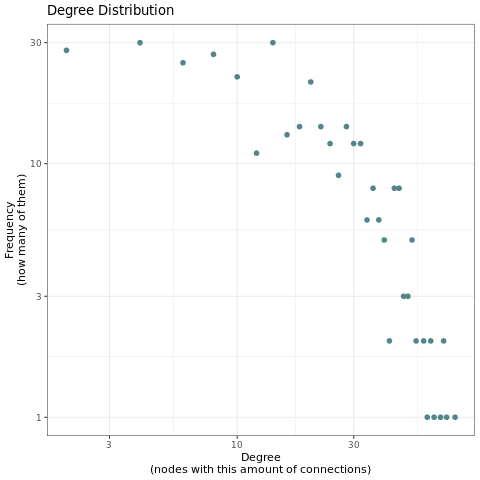
\includegraphics[width=70mm,scale=1.2]{report/figures/degree_distribution.png}

\caption{\textit{Distribución del grado en escala logarítmica}}

\end{center}

En este caso, el coeficiente medio de clustering de nuestra red es de 0.43.
En la figura podemos observar que los nodos con un grado menor varían mucho en cuanto a C, teniendo nodos que están muy agregados y otros que están casi desconectados. Esto no pasa en los hubs, que se mantienen muy cercanos en cuanto a transitividad

\begin{center}

\includegraphics[width=70mm,scale=1.2]{report/figures/clustering_coefficient.png}

\caption{\textit{Coeficiente de clustering}}

\end{center}

Si nos fijamos en la distancia entre los nodos de nuestra red, podemos comprobar que tiene propiedad de mundo pequeño, ya que la mayoría de nodos tienen distancia 3 o 4, siendo la media 3.46.
Es decir, nuestra red está bien comunicada.

\begin{center}

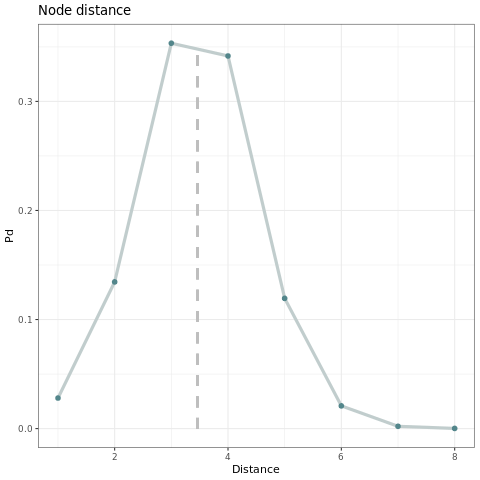
\includegraphics[width=70mm,scale=1.2]{report/figures/Node_distance.png}

\caption{\textit{Distancia entre los nodos}}

\end{center}

En la siguiente figura observamos que la red es bastante robusta ante ataques aleatorios y bastante menos ante ataques dirigidos, lo que nos indica una vez más que el modelo libre de escala es el que se ajusta mejor.

Que disminuya tan rápido la conectividad eliminando una fracción tan pequeña de nos indica que debemos centrarnos en el estudio de esas proteínas principalmente.

\begin{center}

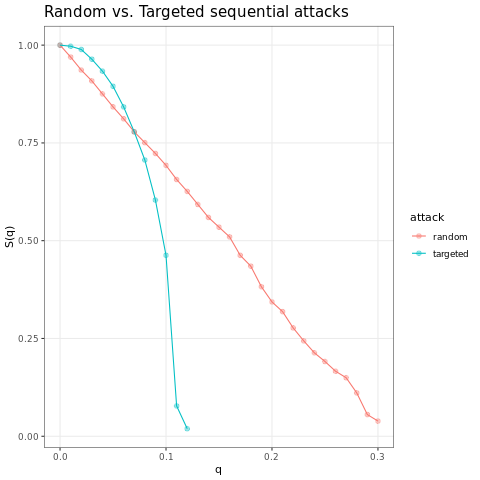
\includegraphics[width=70mm,scale=1.2]{report/figures/sequential_attacks.png}

\caption{\textit{Robustez frente a ataques dirigidos y aleatorios}}

\end{center}

\subsection{Linked Communities}
En esta sección procedemos a obtener las comunidades existentes dentro de nuestra red de proteínas, obtenida en la sección anterior.

Antes debemos tener claro que las comunidades son conjuntos de nodos relacionados entre sí que poseen funciones semejantes y que buscan conseguir un objetivo común. Es por ello por lo que la identificación de las comunidades es un problema relevante para muchas áreas de investigación como la sociología, la biología o la informática.

En general, la comunidades se pueden clasificar en dos tipos, las que están formadas por nodos y las que están formadas por enlaces.

\begin{itemize}
\item Comunidad de nodos: Se tratan de subgrafos formados por nodos densamente conectados entre ellos, pero muy poco conectados con los nodos de alrededor, como se muestra en la imagen. 


\begin{center}

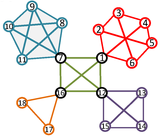
\includegraphics[width=70mm,scale=1.2]{report/figures/nodes.png}

\caption{\textit{Comunidad de nodos}}

\end{center}


\item Link community: Consiste en un subgrafo en el que existe una gran cantidad de enlaces pero muy pocos con las comunidades externas. La forma de detectar estos conjuntos es mediante la división de los enlaces de la red. En estas particiones, las conexiones determinan una comunidad, pero los nodos pueden pertenecer a varias comunidades. 


\begin{center}
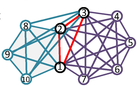
\includegraphics[width=70mm,scale=1.2]{report/figures/links.png}


\caption{\textit{Link community}}

\end{center}

Con esto queremos remarcar que la importancia de la detección de estos subgrafos se debe a que en el campo de la biología, permiten encontrar módulos proteicos con una misma función celular o predecir las funciones de las proteínas.

Por tanto, diseñaremos un código en R que nos permite la detección de las comunidades con el fin de filtrar aquellas que son más importantes (centralidad). De esta forma, podemos llevar a cabo un enriquecimiento funcional de las mismas y así obtener algunas de las funciones celulares que determinan red del SARS-CoV-2.

Además, en el código siguiente se incluyen diferentes gráficas para la visualización de las comunidades.
\end{itemize}

A lo largo de la ejecución del código hemos añadido distintas gráficas para la representación de las comunidades. A continuación se muestra un dendograma de las \textit{link communities}, en el que se puede apreciar una gran cantidad de comunidades. En esta imagen es difícil ver la centralidad de las comunidades, por lo que haremos más representaciones.

\begin{lstlisting}
#link communities dendogram
png(file="linkcomm_dend.png")
plot(proteins.mapped.network.lc, type = "dend")
dev.off()
\end{lstlisting}

\begin{center}
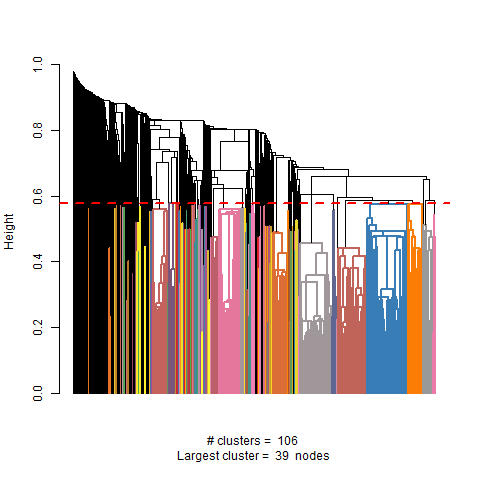
\includegraphics[width=90mm,scale=1]{report/figures/linkcomm_dend.png}


\caption{\textit{Dendograma de Linked Communities}}

\end{center}


Empleando el diseño \textbf{ Fruchterman Reingold} se puede obtener una visión más amplia de las comunidades. 

\begin{lstlisting}
#link communities Fruchterman Reingold layout
png(file="linkcomm_layout.fruchterman.reingold.png")
plot(proteins.mapped.network.lc, type = "graph", layout =
layout.fruchterman.reingold, vlabel=FALSE)
dev.off()
\end{lstlisting}

\begin{center}

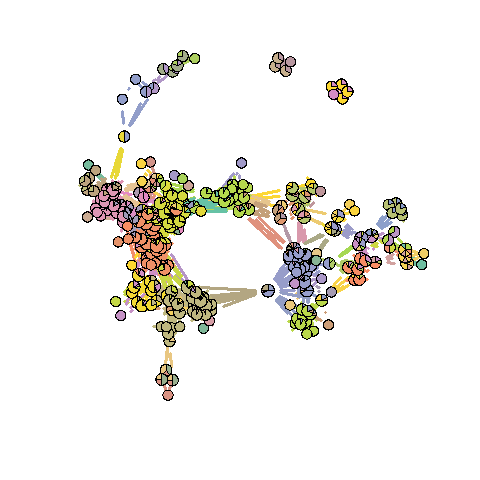
\includegraphics[width=90mm,scale=1]{report/figures/linkcomm_layout.fruchterman.reingold.png}


\caption{\textit{Linked Communities con Fruchterman Reingold layout }}

\end{center}

Sin embargo, lo que nos interesa en este caso es obtener la \textbf{'centralidad comunitaria'} pues se define como la suma de las áreas con mayor influencia sobre los nodos vecinos de la red. Por tanto, nos permite obtener aquellos clusters que ejercen una mayor influencia sobre la red, pudiendo ser determinantes en la funcionalidad de la misma.

Por otra parte, la \textbf{modularidad} consiste en el grado de separación y recombinación existente entre los componentes de una red. Es decir, se considera como una medida de la presencia de estructura comunitaria. Esto permite la búsqueda de comunidades, quedándonos con aquellas que tengan un valor de modularidad positivo y lo más grande posible (modularidad optimizada).

Por ello, hemos calculado la modularidad de las comunidades de nuestra red y hemos representado el valor de la modularidad para cada una de ellas.

\begin{lstlisting}
# Community centrality
community.centrality <- getCommunityCentrality(proteins.mapped.network.lc)

#modularity of the communities
community.connectedness <- getCommunityConnectedness(
proteins.mapped.network.lc,conn = "modularity") 

png(file="communities_modularity.png")
plot(proteins.mapped.network.lc, type = "commsumm", summary = "modularity")
dev.off()
\end{lstlisting}
\begin{center}
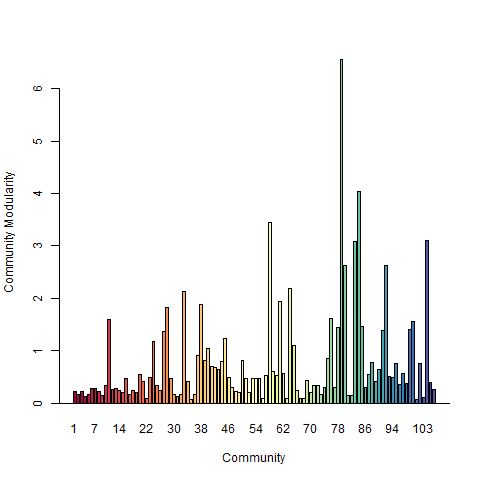
\includegraphics[width=90mm,scale=1]{report/figures/communities_modularity.png}

\caption{\textit{Diagrama de barras de la modularidad de las comunidades}}

\end{center}
En la imagen se observa claramente como hay una comunidad con una modularidad muy alta, lo que indica que esta es más influyente en la red que el resto, concretamente la comunidad 79.


\begin{lstlisting}
# Focus on one linkcomm
#plot one cluster with maximun community modularity
png(file="cluster12_graph.png")
plot(proteins.mapped.network.lc, type = "graph", clusterids =
community.connectedness.maximum, vlabel=FALSE)
dev.off()

\end{lstlisting}

\begin{center}
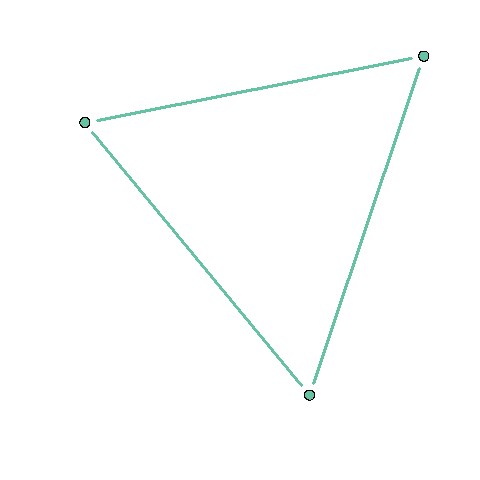
\includegraphics[width=70mm,scale=1]{report/figures/cluster_graph.png}
\end{center}

Por tanto, realizaremos un análisis funcional centrándonos en aquellas comunidades con una modularidad mayor, para determinar si sus funciones moleculares son determinantes o no.

\subsection{Enriquecimiento funcional}
\subsubsection{Cluster 104}

\begin{center}
\vspace{1.5ex}
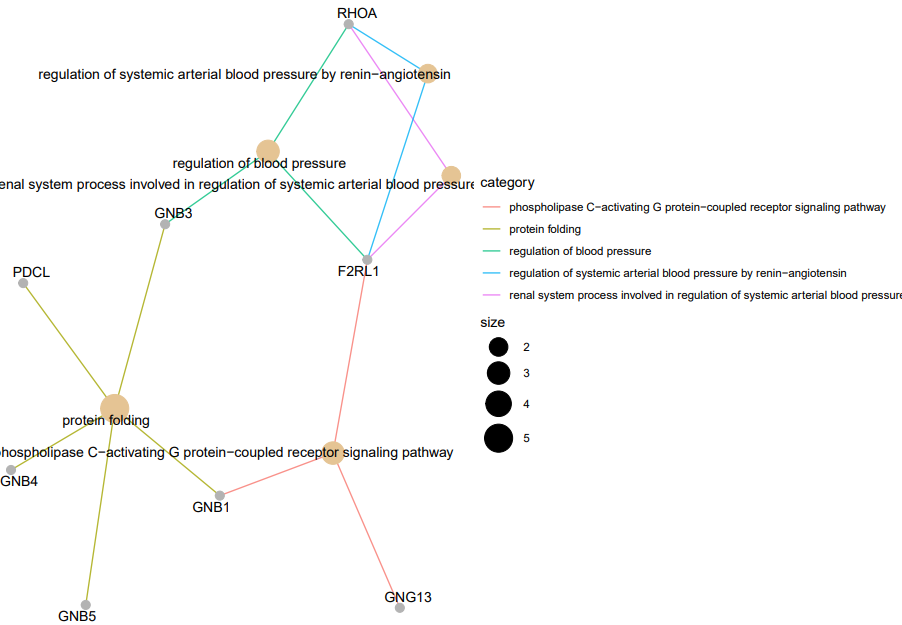
\includegraphics[width=100mm,scale=1.1]{report/figures/enrichGO_heatmap_cnetplot-BP-104-2.PNG}
\vspace{1.5ex}
\end{center}


En la figura superior podemos observar mediante un mapa de calor o heatmap, los 5 términos de la GO predominantes de la subred, además de otras funciones asociadas a cada proteína. 
Para el clúster 104 vemos que el término con un mayor tamaño en el mapa es ‘protein folding’. Esto indica que su GeneRatio (porcentaje de DEGs asociado al término) es grande y el q valor o p valor ajustado, es pequeño.


\begin{center}
\vspace{1.5ex}
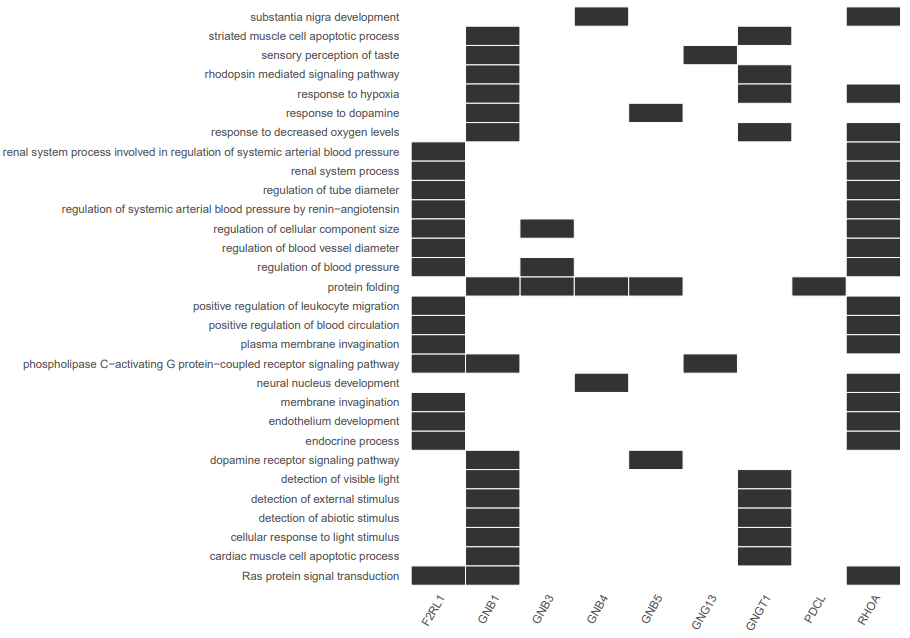
\includegraphics[width=100mm,scale=1.1]{report/figures/enrichGO_heatmap_cnetplot-BP-104-1.PNG}
\vspace{1.5ex}
\end{center}


Investigando en la ontología, obtenemos que el \textbf{plegamiento de proteínas} es un proceso biológico que facilita el ensamblaje de proteínas para dar lugar a una estructura terciaria correcta.


De ahí podemos deducir el papel que juega esta función pues un fallo en plegamiento puede provocar un desorden celular con amplias consecuencias. Es más, existen una gran cantidad de enfermedades generadas por este tipo de fallos como el Alzheimer, el Parkinson, la fibrosis quística y muchos otros trastornos degenerativos, tal y como se mencionan en el artículo \textbf{\textit{‘Protein-misfolding diseases and chaperone-based therapeutic approaches’}}.
Según este estudio, “más de la mitad de las enfermedades humanas podrían estar relacionadas con un plegamiento incorrecto de las proteínas”. Este proceso parece afectar a las chaperonas, pues son las encargadas de reparar las mutaciones que causan las patologías.

Por otra parte, la \textbf{‘ruta de señalización del receptor acoplado a la proteína G que inhibe la fosfolipasa C’}, es otro de los procedimientos identificados en mayor medida con el clúster en cuestión.   Concretamente, esta vía además de inhibir la actividad de la fosfolipasa C, conlleva una disminución de los niveles de DAG y IP3. Este último es un mensajero de señalización celular cuya disminución parece estar relacionada con la \textbf{autofagia} o vía de degradación de proteínas, orgánulos y material citoplasmático. Por su parte, los segundos mensajeros DAG dan lugar a la activación de la proteína quinasa C, la cual permite la activación de una serie de rutas metabólicas que inducen la expresión de proteínas que activan los linfocitos T. Estos desempeñan un papel fundamental en la regulación del sistema inmune, por lo que una alteración de los mismo puede generar una inmunodeficiencia severa.

\begin{center}
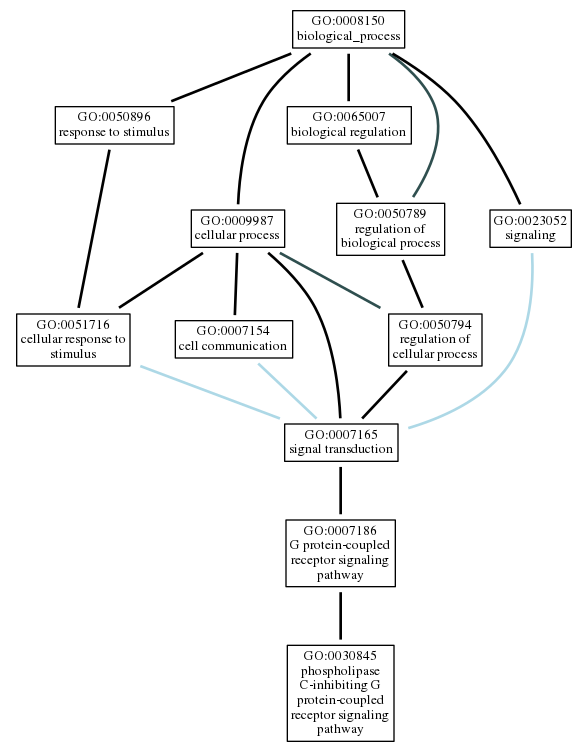
\includegraphics[width=70mm,scale=1]{report/figures/signaling pathway.png}
\end{center}

Otra de las funciones biológicas que aparecen en el enriquecimiento de este módulo, está relacionada con la \textbf{regulación de la presión sanguínea}, y, por tanto, de los niveles de oxígeno. Este es un proceso muy complejo que viene determinado por el Sistema Nervioso Autónomo, el SNC y el riñón. El objetivo del SN es mantener la presión arterial (PA) mediante la regulación de los niveles de oxígeno. Sin embargo, un nivel alto de PA o \textbf{hipertensión}, puede llegar a ser nocivo para el corazón, puesto que lo obliga a bombear más sangre, contribuyendo así al endurecimiento de las arterias, a la producción de accidentes cerebrovasculares, enfermedades renales o insuficiencia cardíaca.

Según un estudio reciente, \textbf{\textit{'COVID-19 and Hypertension: What We Know and Don't Know'}}, el SARS-CV-2 interactúa con el Sistema renina-angiotensina aldosterona (RAAS), actuando sobre el receptor ACE2 induciendo una desregulación de la misma, lo que genera la acumulación lo local de angiotensina II.  Debido a que el sistema RAAS se encarga de regular la presión arterial, la alteración del mismo da lugar a la hipertensión de los pacientes.

\begin{center}
\vspace{1ex}
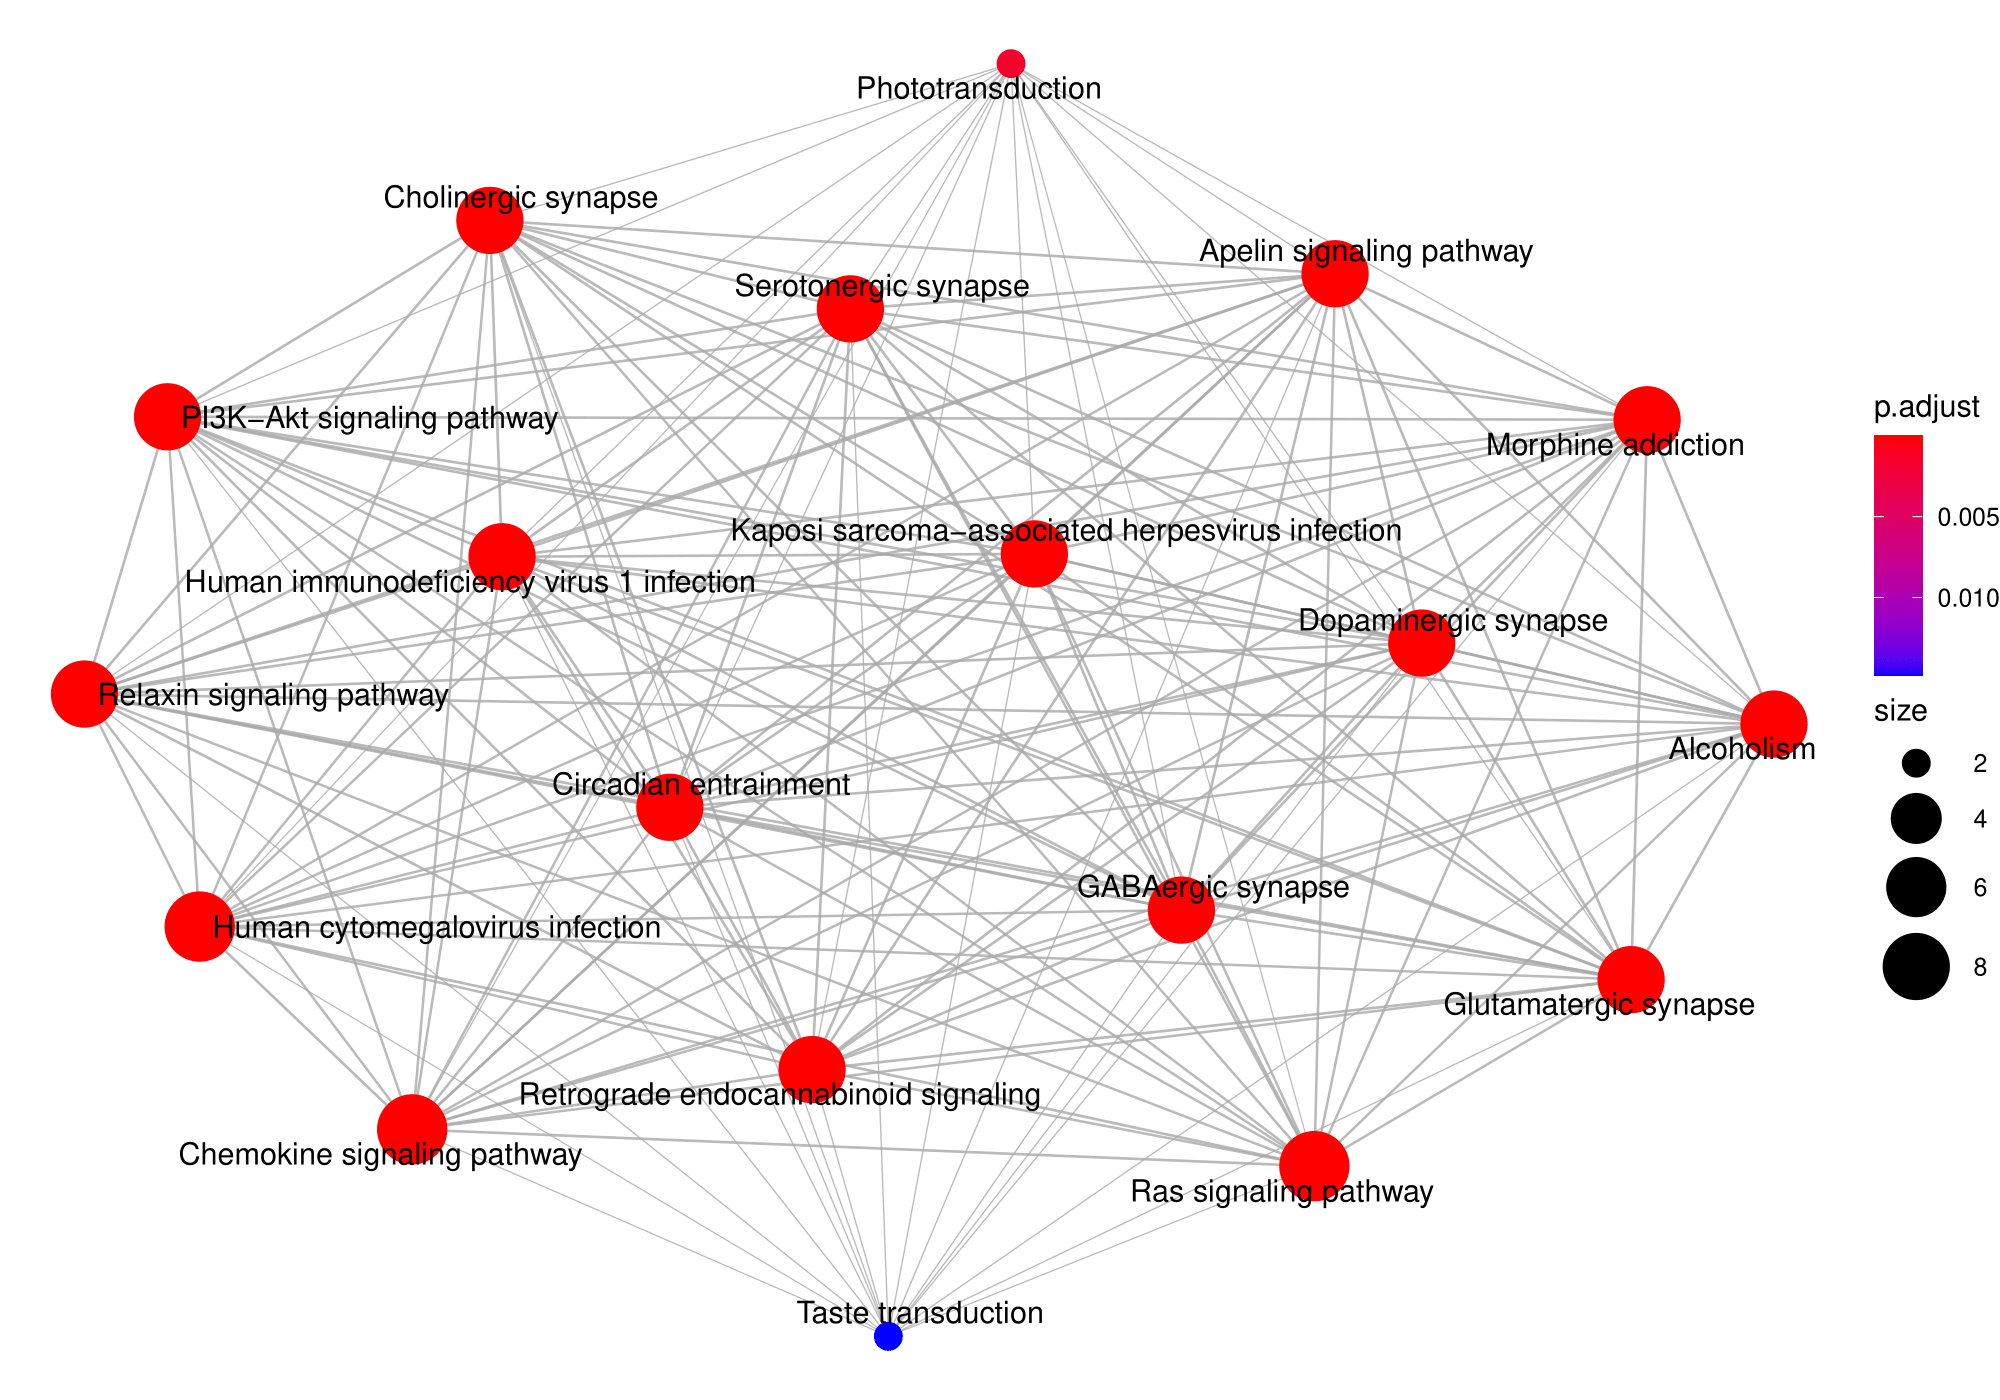
\includegraphics[width=100mm,scale=1]{report/figures/enrichKEGG_enrichmap-BP-104.png}
\vspace{1ex}
\end{center}

Para concluir, en la figura superior podemos observar como alguno de los procesos mencionados se encuentran en el mapa de vías metabólicas. Además, en el mapa de calor obtenido, también se observan muchos de los términos más presentados en el clúster 104.

\subsubsection{Clúster 84}

\begin{center}
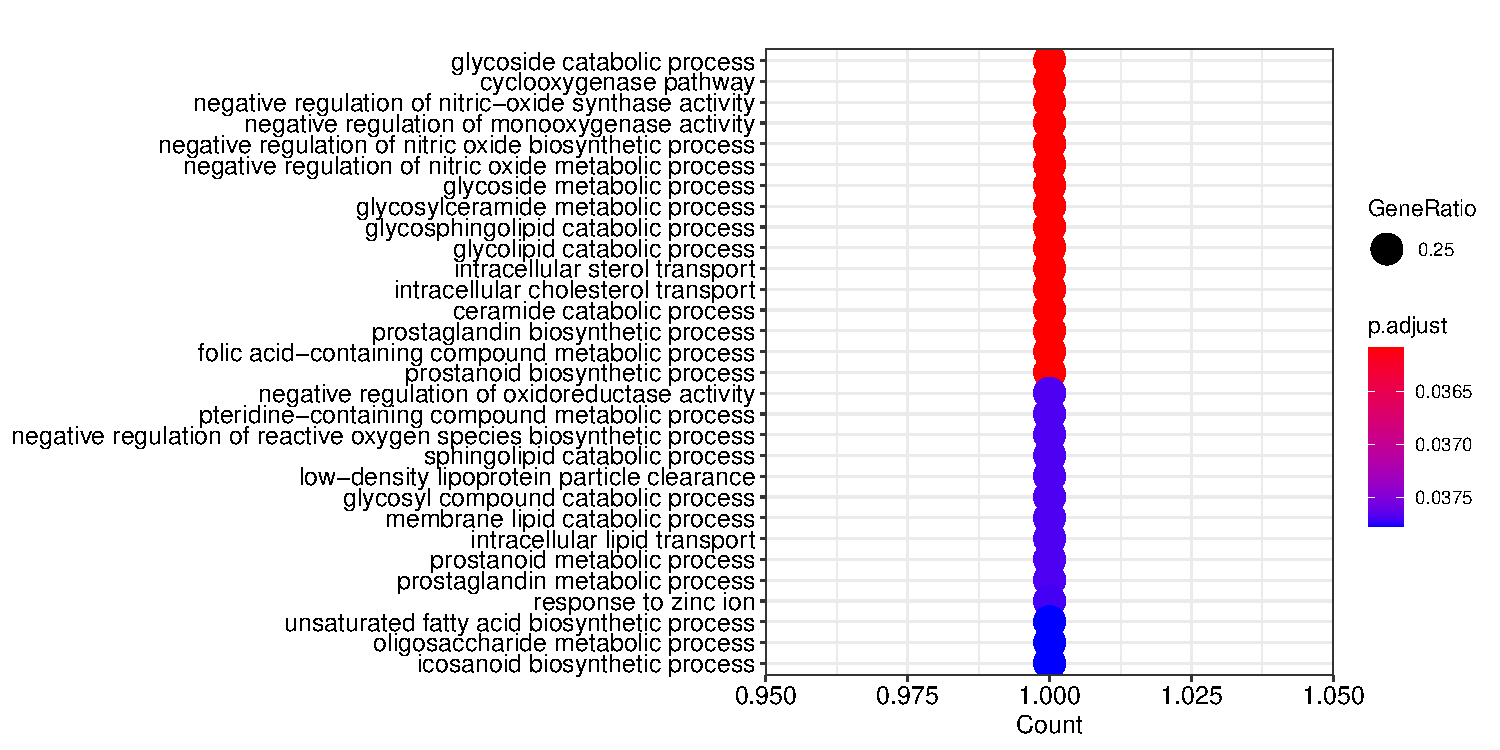
\includegraphics[width=120mm,scale=1]{report/figures/enrichGO_dotplot-BP-84.pdf}
\end{center}

Este clúster está formado por 4 proteínas altamente interconectadas cuyas funciones biológicas se relacionan con 4 aspectos principalmente. El primero de ellos y el más abundante es el \textbf{metabolismo y catabolismo de glúcidos y lípidos}, los cuales son nuestra principal fuente de energía en el organismo. El hecho de que las proteínas del virus interactúen con las de nuestro clúster puede provocar alteraciones en el desarrollo de esta función tan esencial. El siguiente tema a tratar es la \textbf{regulación negativa del óxido nítrico}. Este compuesto es mencionado en varias de las funciones biológicas de nuestras proteínas y se trata de un gas que se genera en el endotelio. Se caracteriza por tener propiedades vasodilatadoras y contribuir al mantenimiento de la presión arterial baja. Por tanto, una regulación negativa del mismo significaría un déficit de este gas en el cuerpo, lo que puede producir entre otras cosas, hipertensión arterial. En tercer lugar en nuestras funciones se hace mención a la \textbf{ruta de la ciclooxigenasa (COX)} y por tanto a sus principales productos que son las \textbf{prostaglandinas}. Éstas son un conjunto de sustancias de carácter lipídico derivadas de los ácidos grasos que conllevan diversos efectos en nuestro organismo, a menudo contrapuestos. Las prostaglandinas afectan y actúan sobre diferentes sistemas, incluyendo el sistema nervioso, el músculo liso y el sistema reproductor. Además, juegan un papel importante en regular diversas funciones como la presión sanguínea, la coagulación de la sangre, la respuesta inflamatoria alérgica y la actividad del aparato digestivo. Por tanto, la interacción del virus con estos compuestos pueden suponer un ataque en nuestro cuerpo. Finalmente aparecen varias funciones relacionadas con el \textbf{transporte intracelular}, lo cual es de vital importancia en las células para expulsar de su interior los desechos del metabolismo o trasladar sustancias que sintetiza como hormonas entre otras actividades.

\begin{center}
\vspace{1.5ex}
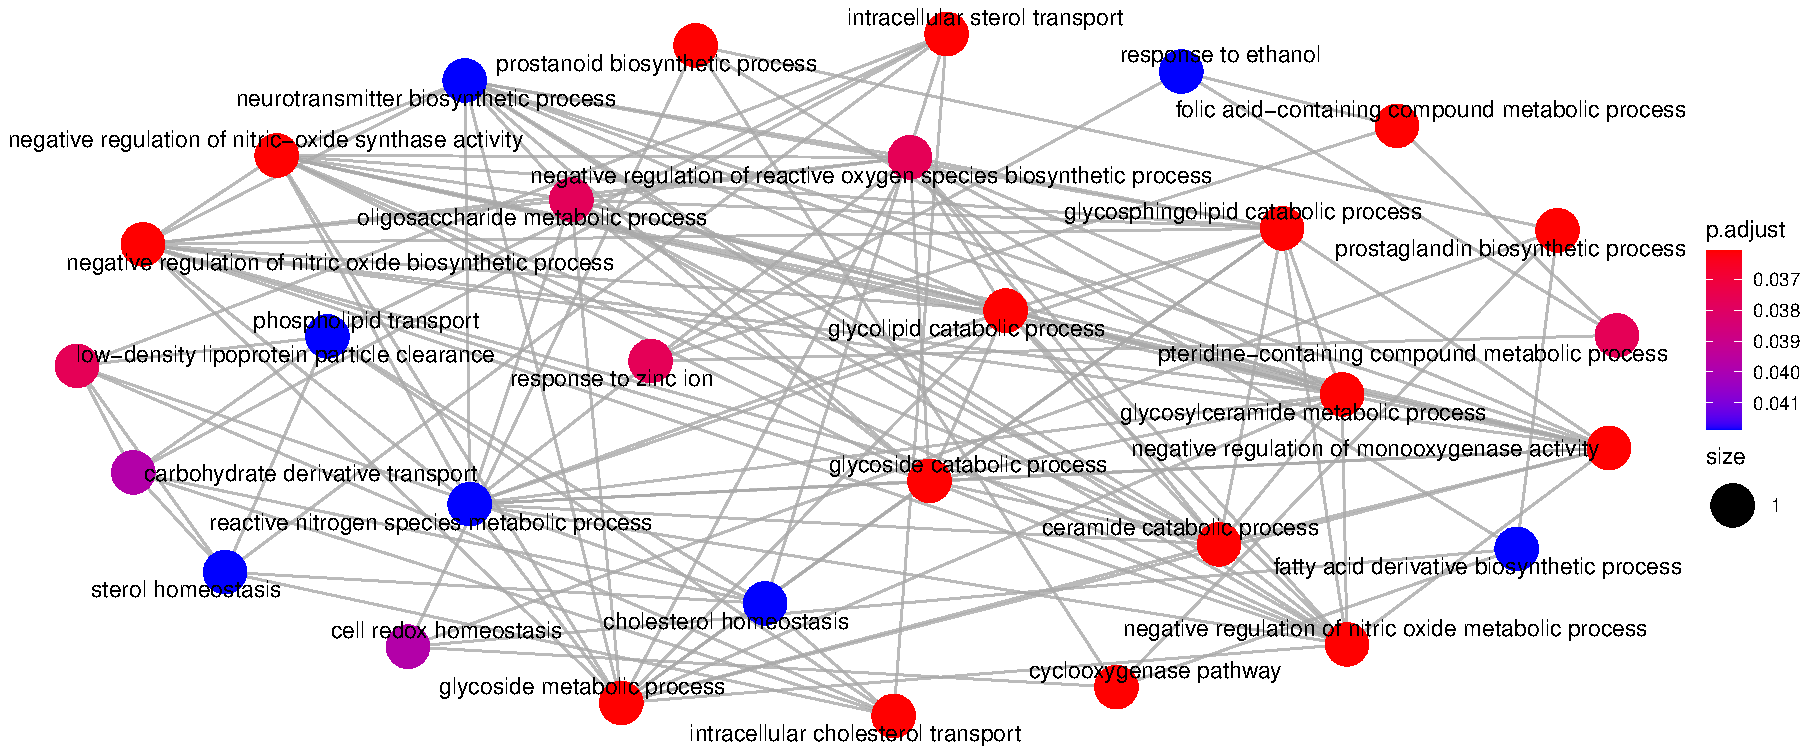
\includegraphics[width=100mm,scale=1]{report/figures/enrichGO_enrichmap-BP-84.pdf}
\vspace{1.5ex}
\end{center}

Además, se puede apreciar como la clasificación de nuestras funciones en estos 4 aspectos se encuentra claramente reflejada en la figura anterior, donde las proteínas pertenecientes a un mismo tema presentan un mayor número de conexiones entre ellas.

\subsubsection{Clúster 79}
La principal funcionalidad que podemos ver es la biosíntesis de las proteínas de membrana GPI: Proteínas de la superficie celular que se pueden unir a la membrana mediante una estructura de glicolípidos denominadas \textbf{anclaje de glicosilfosfatidilinositol (GPI)}. Las proteínas que son detectadas en el cluster con una mayor fiabilidad estadística son las necesarias para la construcción de estas estructuras. Procesos celulares asociados a la biosíntesis de lipoproteínas son atribuidos a dichas proteínas junto con procesos metabólicos de la formación de estos complejos GPI. 

\begin{center}
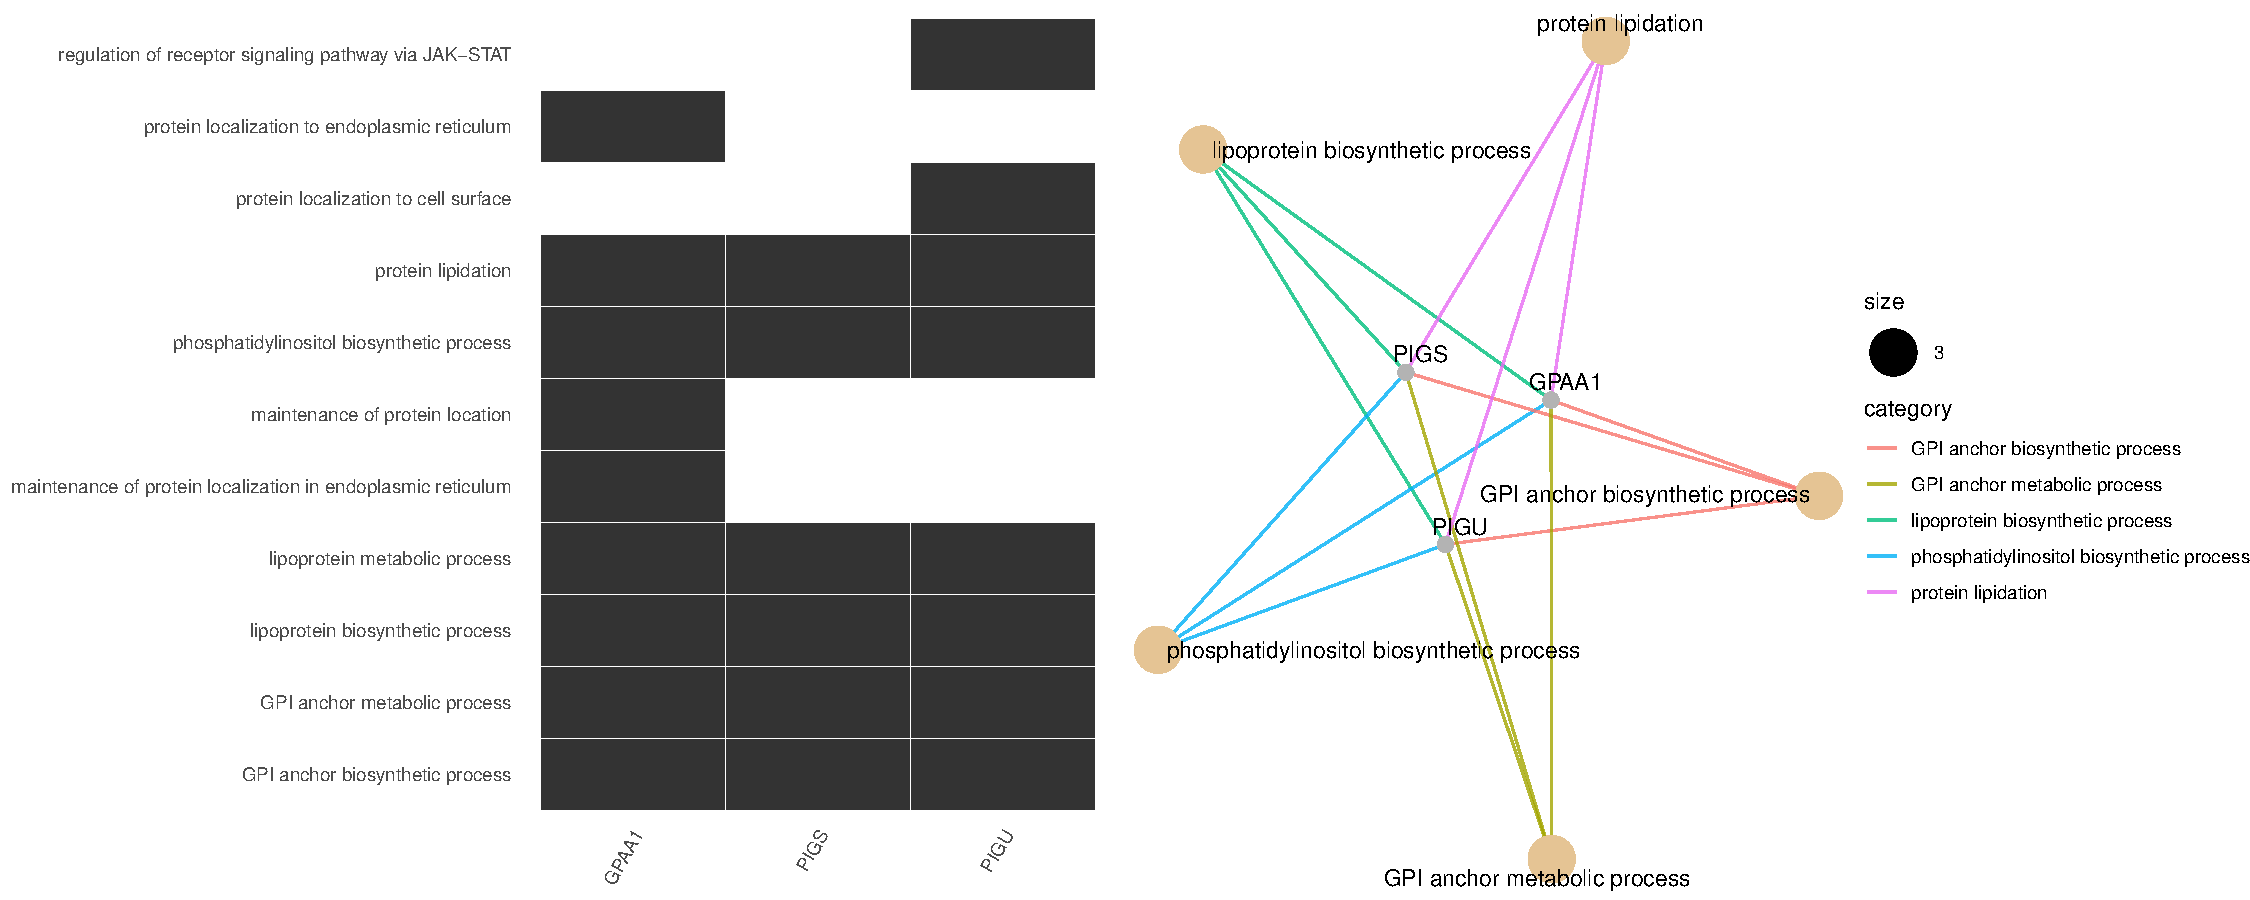
\includegraphics[width=100mm,scale=1.1]{report/figures/enrichGO_heatmap_cnetplot-BP-79.pdf}
\end{center}
\vspace{1.5ex}


Estas estructuras conforman las balsas lipídicas en las membranas celulares las cuales son zonas accedidas por ciertas proteínas del SARS-CoV2, en concreto la proteína \textbf{ORF9c}, la cual podría tratarse de una de las proteínas del coronavirus humano que adquiere un dominio de transmembrana mediante la interacción con estos anclajes y que podría estar asociada con el ataque hacia procesos de señalización inmunológicos. En recientes estudios se muestra cómo ORF9c interactúa con las proteínas de membrana y altera los procesos antivirales en líneas celulares epiteliales pulmonares.

Además se observa que estos componentes son incluso mecanismo de entrada directa en otros virus y se aprecian diferencias en cuanto a estos procedimientos en distintos tipos de coronavirus.

\vspace{1.5ex}
\begin{center}
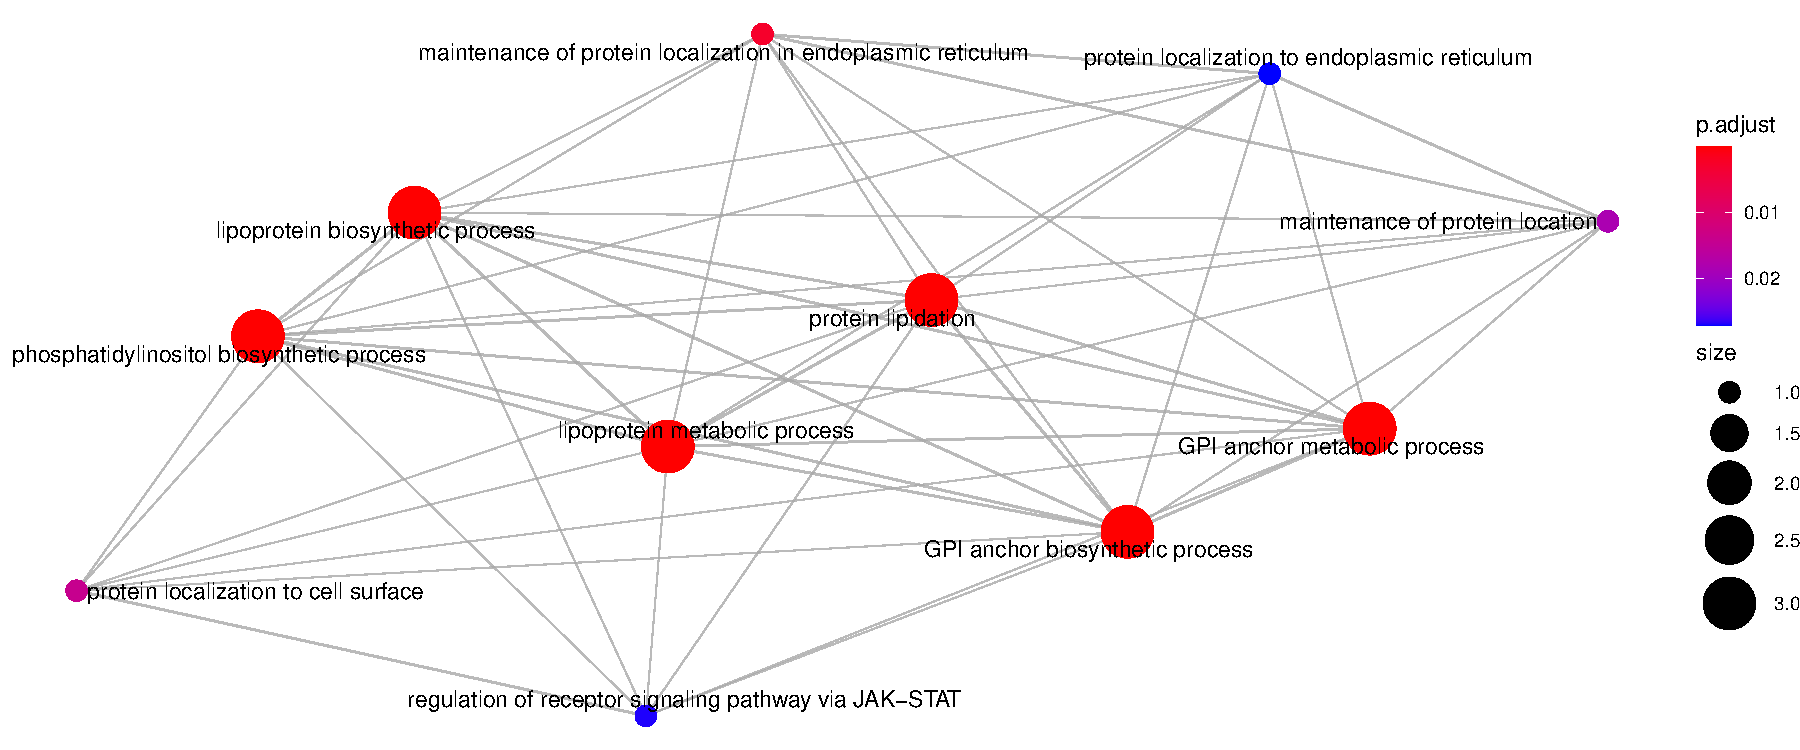
\includegraphics[width=100mm,scale=1.1]{report/figures/enrichGO_enrich_map-BP-79.pdf}
\end{center}
\vspace{1.5ex}

En este caso nuestro análisis de las comunidades proteicas nos ha llevado a concretar la importancia funcional que podría ayudar a estudiar más en profundidad la acción del SARS-CoV2 a partir de un nivel topológico. 


	\section{Discusión}

En este estudio hemos partido de la red de interacciones de proteínas humanas con el SARS-cov2 obtenida en \textbf{\textit{‘A SARS-CoV-2 protein interaction map reveals targets for drug repurposing’}} y la hemos \textbf{ampliado hasta obtener 425 interacciones}. Tras eliminar los nodos no conectados, hemos obtenido una componente conexa de 395 nodos. A partir de este grafo hemos aplicado diversas herramientas con el objetivo de obtener más información acerca de su naturaleza, como se ha comentado en el apartado de resultados.


Mediante un \textbf{enriquecimiento funcional} de las 4 comunidades más centrales de nuestra red hemos podido conocer los principales procesos biológicos, funciones moleculares y componentes celulares a los que se asocian las proteínas estudiadas. Tal y como se comenta en  \cite{Gysi2020NetworkCOVID-19}, diversos procesos se relacionan con la actividad cardiovascular del organismo, llegando a provocar desordenes en la presión arterial o en el sistema renina-angiotensina-aldosterona. Esto también lo hemos podido comprobar al estudiar el clúster 84, pues provoca una regulación negativa del óxido nítrico, un compuesto que contribuye a la regulación de la presión arterial.


Otra función que hemos podido descubrir es la participación en la síntesis de lipoproteínas formando los complejos GPI, que permiten el ataque a los procesos de señalización inmunológica. De ahí podemos deducir la efectividad de este virus que es capaz de provocar una inmunodeficiencia severa. Además, la forma en que el virus se propaga en el organismo es particular del SARS-CoV-2.


Finalmente, gracias a la \textbf{búsqueda en Drugbank} no solo hemos podido analizar los medicamentos que se dirigen a las proteínas de nuestra red, sino también nos permite interpretar el mecanismo de acción de los mismos. Por ejemplo, la pravastina podría disminuir las probabilidades de mortalidad del paciente pues es un fármaco que previene el ataque del virus sobre el corazón, mientras que la teofilina podría ayudar a combatir la grave neumonía que provoca el virus en cuestión. 


Además, hemos comprobado cómo los anestésicos volátiles pueden ser una nueva alternativa para la sedación e intubación de pacientes gravemente afectados por el Covid-19 y que efectos puede tener sobre la probabilidad de muerte de los mismos.


	\section{Conclusiones}

Tras contemplar y discutir todos los resultados obtenidos durante el desarrollo de nuestro estudio cabe mencionar la alta conectividad y \textbf{mantenimiento de coherencia} entre las distintas fases del proceso. Se puede apreciar como los módulos más importantes de nuestra red han sido los que finalmente han permitido descubrir las funciones moleculares y procesos biológicos más trascendentales respecto a la interacción del virus en nuestro organismo. Además, estas funciones fueron claramente confirmadas en apartados posteriores cuando el estudio llevado acabo sobre DrugBank nos proporcionaba una serie de medicamentos cuyos objetivos se centraban en tratar muchas de las consecuencias que estas funciones podían acarrear sobre nuestra salud. Es decir, los descubrimientos llevados a cabo durante este trabajo han mantenido en todo momento una dirección muy definida que nos ha permitido realizar afirmaciones sólidas y cómodamente contrastadas.

Además, la conclusión más importante que cabe mencionar de este trabajo es sin duda la gran cantidad de información útil que nos puede ofrecer el estudio de un interactoma concreto cuando ha sido correctamente acotado y seleccionado bajo condiciones coherentes. En nuestro caso, estudiar la porción del \textbf{interactoma humano} asociado al virus SARS-CoV-2, nos ha permitido conocer no sólo las funciones de las proteínas humanas, sino que a través de dicha información ser capaces de descubrir las posibles interacciones del virus con nuestro organismo, las posibles consecuencias clínicas de dicha interacción, características del propio virus y por último qué medicamentos pueden llegar a ser más efectivos para luchar contra el mismo. Es decir, la red estudiada en este trabajo ha conseguido actuar como una especie de espejo sobre el que hemos podido analizar el reflejo de las partes más esenciales de nuestro virus de interés.

Es evidente que cuantos más trozos de este espejo metafórico tengamos, mayor será la claridad y la precisión con la que podamos analizar el virus y por tanto mayor será el conocimiento que tengamos sobre el mismo. Con esto, queremos señalar la gran importancia que tiene seguir descubriendo nuevos elementos y conexiones del interactoma humano, ya que actualmente se afirma que nuestro conocimiento sobre el mismo es aproximadamente de un 10\%. Ampliar esta gran red o incluso llegar a completarla nos permitiría sin lugar a dudas obtener una mayor cantidad de información con la que poder realizar análisis más profundos y efectivos. Esto también se extendería a estudios más concretos como el nuestro, ya que poseer el interactoma completo asociado al SARS-CoV-2 nos abriría las puertas a nuevos descubrimientos incluidos aquellos que nos permitan eliminar su actual amenaza.

	\section{Anexos}

\subsection{Flujo de trabajo en BASH}

Hemos planteado el flujo de BASH de la siguiente manera:
Tendremos un archivo principal \textit{launch.sh} que se ejecuta desde la consola pasándole como parámetro la ruta de la carpeta donde se guardarán los resultados. Este comprobará si están instalados los paquetes necesarios para la ejecución del código. Si estos están instalados en la carpeta \textit{software/deps-r} (Porque ya se haya ejecutado previamente el archivo \textit{setup.sh}), se ejecutará directamente el archivo \textit{human-covid-network.R}. La ejecución del archivo mostrará resultados numéricos, como el diámetro de la red, por pantalla y generará gráficos en formato PNG y PDF. 

\begin{center}

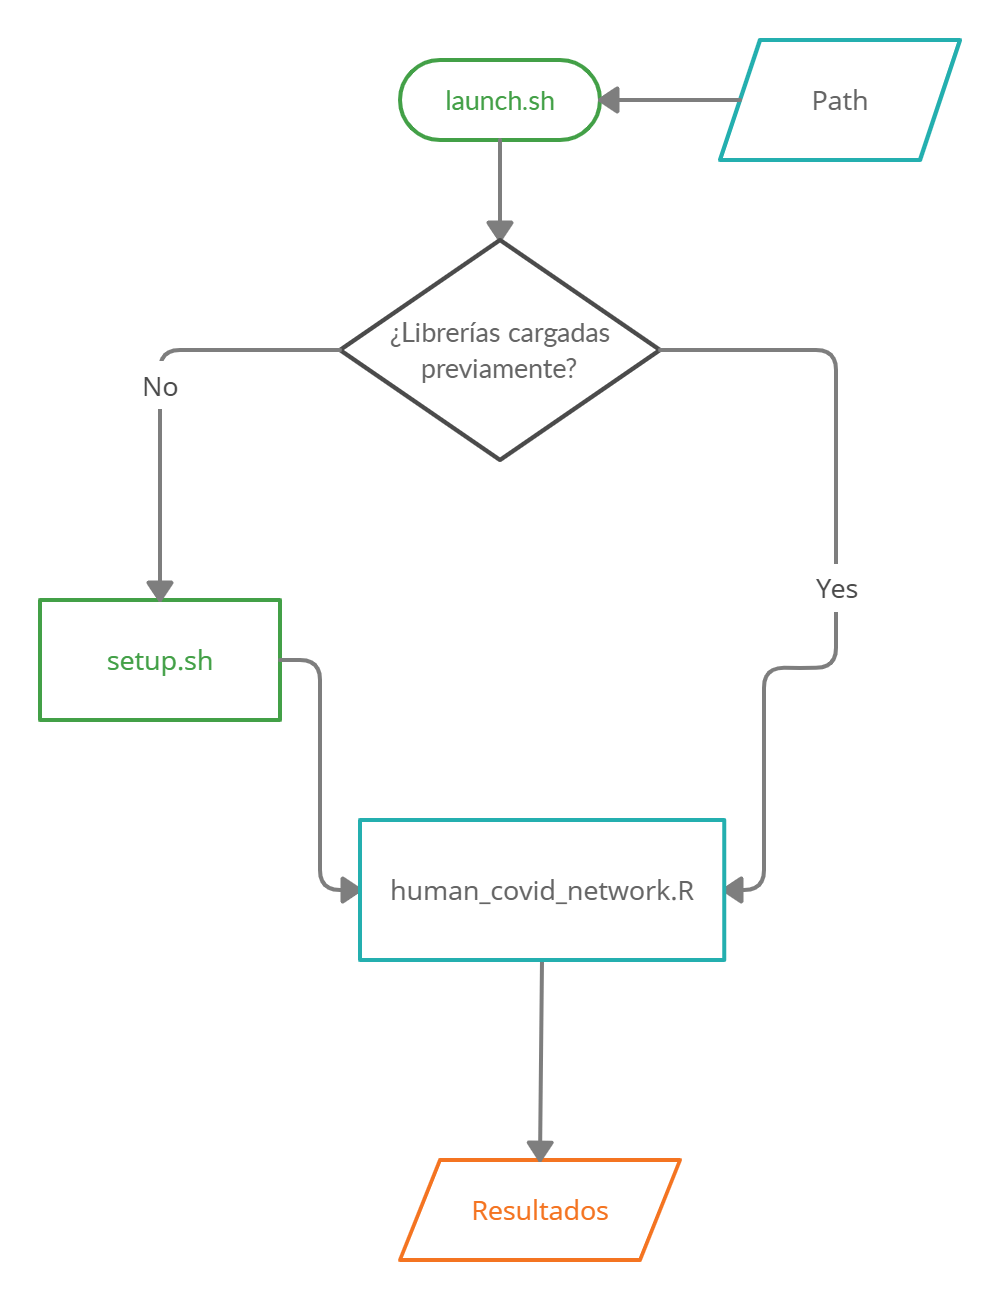
\includegraphics[width=90mm,scale=1]{report/figures/flujo.PNG}

\end{center}

\subsection{Ejecución}
Es necesaria la ejecución desde un terminal Linux, ya que algunas de las librería que se han utilizado para realizar este trabajo solo pueden instalarse desde ahí.
Además, deberemos disponer de la versión 4.0 o superior de R para poder acceder a la versión más actualizada de STRINGdb(Si se usa una versión anterior se generaran resultados distintos a los expuestos en esta memoria.

	
	%%%%%%%%%%%%%%%%%%%%%%%%%%%%%%%%%%%%%%%%%%%%%%
	%% OTRA INFORMACIÓN                         %%
	%%%%%%%%%%%%%%%%%%%%%%%%%%%%%%%%%%%%%%%%%%%%%%
	
	\begin{backmatter}
	\newpage
		\section*{Abreviaciones}%% if any
			
		
		\section*{Disponibilidad de datos y materiales}%% if any
			https://github.com/Fiorellaps/project\_template
		
		\section*{Contribución de los autores}
			S.C.L : Encargada del Enriquecimiento funcional de los clústers más centrales de la red en R y en el documento y creación de launch.sh; F.P.S: Escritura de abstract, introducción, resultados (Linked Communities), discusión y obtención de LC en R; A.S.O: Búsqueda de la red de interacción PPI, escritura de resultados (Enriquecimiento Funcional) y conclusión.; MR.V:P: Búsqueda de medicamentos en Drugbank, análisis inicial y robustez, creación de setup en bash y escritura de resultados (Búsqueda de Drugbank y análisis inicial y robustez).
		
		
		%%%%%%%%%%%%%%%%%%%%%%%%%%%%%%%%%%%%%%%%%%%%%%%%%%%%%%%%%%%%%%%%%%%%%%%%%%%%%%%%%%%%%%%%
		%% BIBLIOGRAFIA: no teneis que tocar nada, solo sustituir el archivo bibliography.bib %%
		%% por el que hayais generado vosotros                                                %%
		%%%%%%%%%%%%%%%%%%%%%%%%%%%%%%%%%%%%%%%%%%%%%%%%%%%%%%%%%%%%%%%%%%%%%%%%%%%%%%%%%%%%%%%%
		
		\bibliographystyle{vancouver} % Style BST file (bmc-mathphys, vancouver, spbasic).

		 \typeout{\bibliography{bibliography/bibliography.bib}}     
         \bibliography{bibliography/bibliography}
         \nocite{*}
	\end{backmatter}
\end{document}
